\documentclass{article}
\usepackage[final]{neurips}
\usepackage[utf8]{inputenc} 
\usepackage[T1]{fontenc}   
\usepackage{hyperref}    
\usepackage{url}           
\usepackage{booktabs}      
\usepackage{amsfonts}      
\usepackage{mathtools}
\usepackage{amssymb}
\usepackage{float}
\usepackage{nicefrac}       
\usepackage{microtype}     
\usepackage[shortlabels]{enumitem}
\usepackage{xcolor}
\usepackage{graphicx}
\usepackage{fourier}	
\usepackage{xepersian}
\settextfont{XB Yas.ttf}

%------------------------------------------------------------------------------
\title{\lr{User Story}}

\author{
	مریم سعیدمهر \\
	شماره دانشجویی : ۹۶۲۹۳۷۳
	\and
	ساجده نیک نداف \\
	شماره دانشجویی : ۹۶۳۷۴۵۳
	\and
	مرضیه علیدادی \\
	شماره دانشجویی : ۹۶۳۱۹۸۳
}

\begin{document}	
%------------------------------------------------------------------------------
\begin{minipage}{0.1\textwidth}
	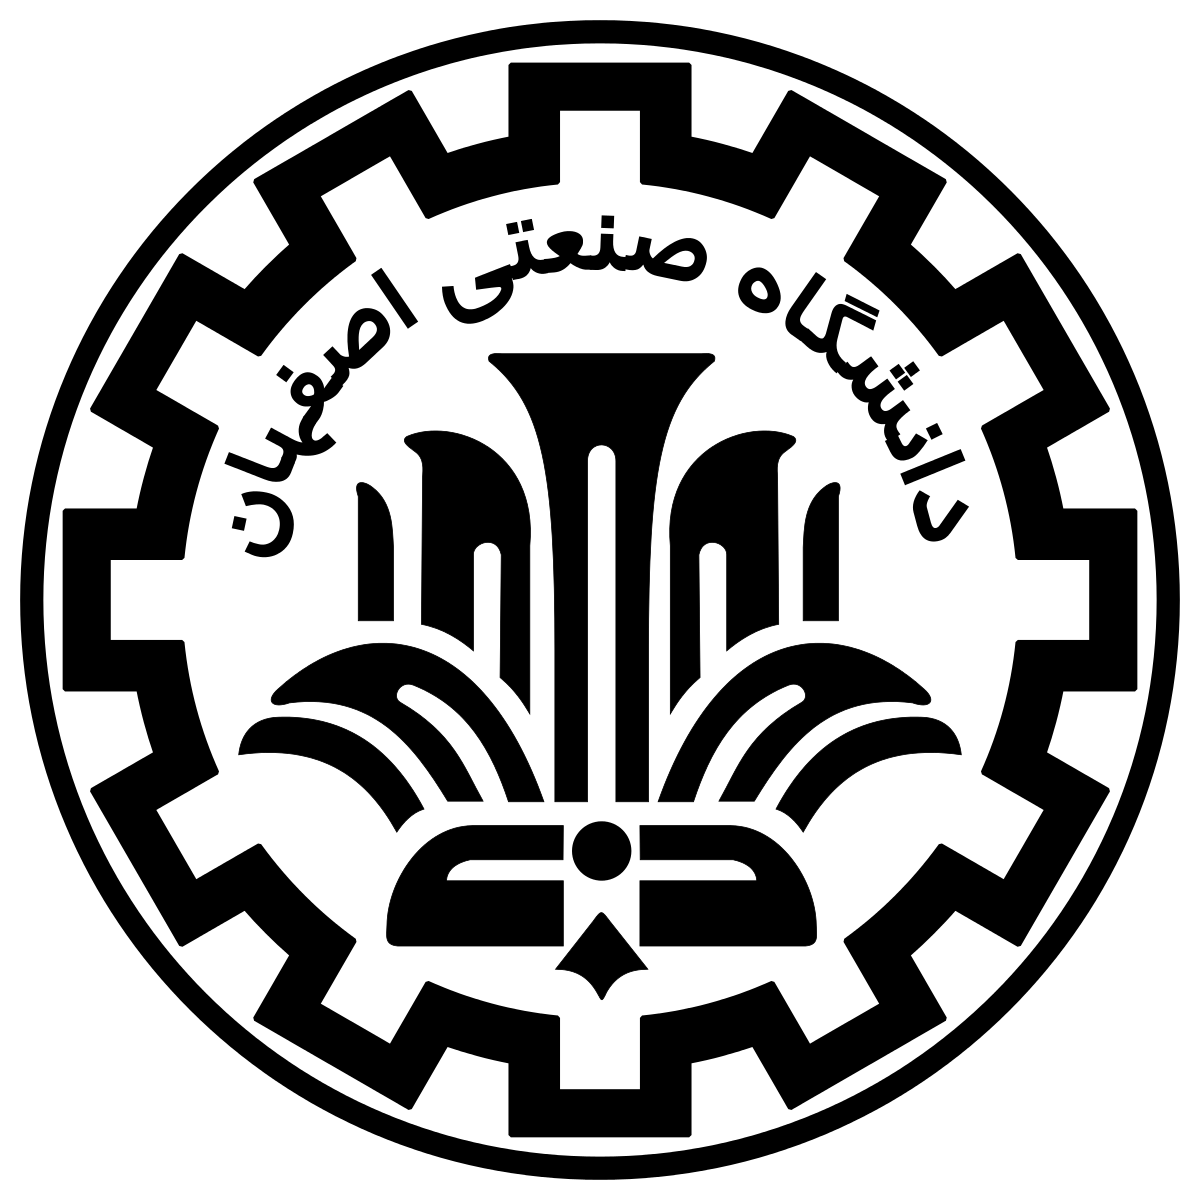
\includegraphics[width=1.1cm]{Pic/IUT.png}
\end{minipage}
\hfill
\begin{minipage}{0.9\textwidth}\raggedleft
دانشگاه صنعتی اصفهان\\
مهندسی نرم افزار ۲ (نیمسال دوم ۱۳۹۹)\\
\end{minipage}

\makepertitle

%------------------------------------------------------------------------------
\section{کاربر}
\begin{itemize}
	\item من به عنوان کاربر میخواهم در سامانه \lr{sign up} کنم تا یک اکانت شخصی داشته باشم.
	\\
کاربر باید نام، نام خانوادگی، شماره موبایل، ایمیل و نام کاربری و دوبار رمزش را وارد کند. رمزش باید حداقل دارای طول ۸ کاراکتر باشد.	

	\item من به عنوان کاربر میخواهم در سامانه login کنیم تا به اکانت شخصی ام دسترسی ایمن پیدا کنم.
	\\
اگر کاربر رمز و نام کاربری خود را درست وارد کرده باشد، یک توکن دریافت کند و وارد حساب کاربری خود شود. اگر کاربر رمز یا نام کاربری خود را اشتباه وارد کرده بود، با پیغام خطا مواجه شود.

	
	\item من به عنوان کاربر میخواهم در پایان کار با سامانه ، به شکلی ایمن از سامانه logout کنم.
	\\
باید توکنی که کاربر دارد باطل شود و از حساب کاربری خود خارج شود. و باید دفعات دیگر که می‌خواهد وارد حساب خود شود، دوباره لاگین انجام دهد.

	\item من به عنوان کاربر میخواهم به لیستی از تمام فایل های بارگذاری شده در سامانه دسترسی داشته باشم تا بتوانم از بین آنها فایلی را انتخاب کنم.
	\\
در صفحه ی اول سایت، یک لیست از همه ی فایل ها باید وجود داشته باشد.

	\item من به عنوان کاربر میخواهم فایلی که انتخاب کرده ام را خریداری کنم تا بتوانم به محتوای آن دسترسی داشته باشم.
	\\
کاربر باید یک فابل را انتخاب کند و گزینه ی خرید را انتخاب کند و به اندازه ی هزینه ی فایل، از شارژ کیف پول او کم شود و آن فایل برایش خریداری شود. اگر موجودی کیف پول کاربر برای هزینه ی فایل انتخابی کافی نبود، خطا دریافت کند.

	\item من به عنوان کاربر میخواهم یک لیست از جدیدترین فایل‌های بارگذاری شده ببینم تا درجریان آخرین به روزرسانی ها باشم.
	\\
در صفحه ی اصلی، بخشی وجود داشته باشد که جدید ترین فایل های بارگذاری شده در سایت را به کاربر نشان دهد.

	\item من به عنوان کاربر میخواهم یک لیست از محبوب‌ترین فایل‌های بارگذاری شده ببینم تا به محبوب‌ترین‌ فایل‌ها دسترسی داشته باشم.
	\\
در صفحه ی اصلی، بخشی وجود داشته باشد که محبوب ترین فایل های بارگذاری شده  بر اساس نظر کاربران در سایت را به کاربر نشان دهد.

	\item من به عنوان یک کاربر میخواهم به جزئیات و اطلاعات هر فایل دسترسی داشته باشم تا بتوان فایل دلخواهم را هوشمندانه تر انتخاب کنم.
	\\
در هر لیستی با کلیک روی نام فایل مشخصات آن از قبیل نویسنده ، دسته بندی ، تگ ها، توضیحات ، فرمت فایل، قیمت، حجم آن و … نمایش داده شود.
	
	\item من به عنوان کاربر میخواهم هر فایل امتیازدهی مناسبی داشته باشد تا در انتخاب فایل موردنظرم بین محتواهای مشابه ، فایل مناسب تر را پیدا کنم.
	\\
در صفحه ی اطلاعات فایل چنانچه کاربر فایل را خریداری کرده باشد بتواند به محتوا و کیفیت آن از یک تا پنج امتیاز دهد.

	\item من به عنوان کاربر میخواهم بعد از انتخاب و خریداری فایل موردنظرم بتوانم به سهولت آن را بارگیری کنم تا خارج از محیط سامانه نیز به فایل های خریداری شده ام دسترسی داشته باشم.
	\\
چنانچه کاربر فایل را خریداری کرده بود بتواند آن را بارگیری کند و بارگیری به طور کامل انجام شود و فایل به درستی دریافت شود و اگر فایل را خریداری نکرده بود این گزینه به کاربر نشان داده نشود

	\item من به عنوان کاربر میخواهم فایل(ها)ی جدیدی را در سامانه بارگذاری کنم تا بتوانم فایل هایم را برای فروش یا به صورت رایگان در اختیار سایرین قرار دهم.
	\\
کاربر بتواند اطلاعات فایل خود مانند اسم فایل، توضیحات، دسته بندی، تگ ها ، قیمت و خود فایل را وارد کرده و با تایید، فایل به لیست فایل های بارگذاری شده ی سایت اضافه شود

	\item من به عنوان کاربر میخواهم در پروفایل شخصی ام برخی مشخصات کاربری ام را وارد ، تغییر یا حذف کنم تا بتوانم اطلاعات اکانتم را بروز و صحیح نگه دارم. 
	\\
کاربر گزینه ویرایش در صفحه کاربری خود داشته باشد و بتواند اطلاعاتی مثل نام و .. را تغییر دهد

	\item من به عنوان یک کاربر میخواهم به کلیه فایل هایی که خریداری کرده ام دسترسی داشته باشم تا شخصاً نیازی به جمع آوری فایل های خریداری شده ام نداشته باشم.
	\\
کاربر در صفحه ی کاربری خود باید بخشی داشته باشد که بتواند لیستی از فایل هایی که تا الان خریداری کرده است را مشاهده کند

	\item من به عنوان کاربر میخواهم به کلیه فایل هایی که در سامانه بارگذاری کرده ام دسترسی داشته باشم تا بتوانم مدیریت بهتری روی آنها داشته باشم.
	\\
کاربر در صفحه ی کاربری خود باید بخشی داشته باشد که بتواند لیستی از فایل هایی که تا الان بارگذاری کرده است را مشاهده کند

	\item من به عنوان کاربر میخواهم به امتیاز سایر کاربران به تک تک فایل هایی که در سامانه بارگذاری کرده ام اشراف  داشته باشم تا از عملکردم اگاه باشم.
	\\
کاربر در پنل کاربری باید بتواند به امتیازاتی که سایر کاربران به فایل های بارگذاری شده اش نسبت داده اند دسترسی داشته باشد

	\item من به عنوان کاربر میخواهم ترتیب نمایش فایل هایی که در سامانه بارگذاری کرده ام را بر اساس شاخص هایی نظیر محبوبیت یا تاریخ ، تغییر دهم تا اشراف کامل بر مدیریت فایل هایم داشته باشم.
	\\
کاربر در پنل کاربری اش باید بتواند روی ترتیب نمایش فایل های بارگذاری شده اش ، فیلترهای مناسبی اعمال کند

	\item من به عنوان کاربر میخواهم سابقه تراکنش هایی که با کیف پول مجازی ام داشته ام را در دسترس داشته باشم تا بتوانم امور مالی ام را بهتر مدیریت کنم.
	\\
کاربر در پنل کاربری اش باید بتواند به تمام سوابق تراکنش های کیف پولش از قبیل شارژ و پرداخت ، دسترسی کامل داشته باشد

	\item من به عنوان کاربر میخواهم از طریق اکانت شخصی ام در سامانه ، بتوانم کیف پولم را به شکل مطمئنی شارژ کنم.
	\\
کاربر در پنل کاربری خود و قسمت کیف پول ، باید بتواند در هر زمان به درگاه بانک به شکل ایمن متصل شده و کیف پولش را شارژ کند

	\item من به عنوان کاربر میخواهم حق مولف محفوظ بماند تا از جنبه مالی و معنوی متضرر نشوم.
	\\
سیستم باید به طور خودکار ، بعد از بارگذاری فایل های جدید یک امضای دیجیتال با روش های رمزنگاری یا نهان نگاری دیجیتال ، به فایل اضافه کند تا حق ناشر محفوظ بماند و سایرین نتوانند دست به نشر غیرمجاز آثار بزنند

	\item من به عنوان کاربر میخواهم فایل (های) مورد نیازم را با جستجوی نام یا دسته بندی آن پیدا کنم.
	\\
هرکاربر باید بتواند فایل مورد نیاز خود را با جستجوی نام یا دسته بندی یا تگ های موردنظرش ، در سیستم پیدا کند	
\end{itemize}

\end{document}
